\chapter{Programming Principles}
%Aufgabe: Analyse und Begründung für 5 der vorgestellten Prinzipien (SOLID/GRASP/DRY/KISS/YAGNI/Conway)
\section{Dependency Inversion Principle}
\label{chap:dip}
Das Dependency Inversion Principle (kurz: DIP) besagt, dass Module hoher Ebenen nicht von Modulen niedriger Ebenenen abhängen sollten. Stattdessen sollten beide von Abstraktionen abhängen. Weiterhin sollten Abstraktionen nicht von Details abhängen, sondern umgekehrt.\\
Ein Beispiel hierfür sind die ApplicationServices, deren einzige Abhängigkeit zur Domain-Schicht in der Verknüpfung mit dem entsprechenden Domain-Repository-Interface (also der Abstraktion des Repositories) liegt. Die eigentliche Verknüpfung erfolgt zur Laufzeit über eine Injection durch die @Autowired-Annotation von Spring Boot.
\vspace*{0.5cm}
\begin{figure}[!htb]
    \centering{
        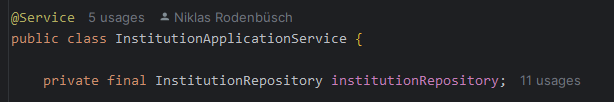
\includegraphics[width=14cm]{images/dip.png}}
    \caption[Dependency Inversion Principle]{DIP-Beispiel anhand der Klasse InstitutionApplicationService}
    \label{fig:dip}
\end{figure}

\section{Low Coupling}
Der Begriff \q{Kopplung} gilt als Maß für die Abhängigkeit einer Klasse von ihrer Umgebung. Das Prinzip \q{Low Coupling} besagt also, dass die Kopplung von Klassen so niedrig wie möglich gehalten werden sollte. Ein Beispiel aus der Anwendung ist die Persistence-Schicht. Die einzigen Klassen, die direkt mit dieser Schicht zusammenarbeiten, sind die \q{RepositoryBridges} Persistence-Schicht. Somit könnte beispielsweise die Datenbank ausgetauscht werden, ohne dafür große Teile der Anwendung ändern zu müssen.

\section{High Cohesion}
Hohe Kohäsion ist ein Maß für den inneren Zusammenhalt einer Klasse, also wie \q{eng} Methoden und Attribute einer Klasse zusammenarbeiten. Dieses Prinzip wurde beispielsweise durch die Implementierung des ValueObjects \q{AccountOwnerNameValue} berücksichtigt, das den Namen eines Account Besitzers enthält. Da der Name eines Account Besitzers an sich nichts mit den anderen Eigenschaften eines Accounts zu tun hat, erhöht die Einführung des ValueObjects die Kohäsion.
%ValueObject

\section{Indirection}
Das Prinzip \q{Indirection} bezeichnet das Delegieren von Aufgaben an andere Objekte und Klassen. Ein Beispiel aus der Anwendung hierfür sind die Methoden der Domain-Repositories (siehe Abb. \ref{fig:indirection}) die ihre eigentlichen Aufgaben lediglich an die JPA-Repositories weitergeben.

\section{Controller}
Der Controller ist das erste Objekt hinter der UI, das Anweisungen annimmt und kontrolliert. Er ist quasi die \q{Steuereinheit} des Programms. Der Controller ist in der Regel der einzige Ansprechpartner, den die UI hat. Er empfängt dabei Anweisungen von der UI und delegiert diese, ohne viel eigene Funktionalität zu implementieren, an Domain-Objekte und Services weiter.\\
Beispiele für Controller in der Anwendung sind die REST-Controller-Klassen der API-Schicht.

\begin{figure}[!htb]
    \centering{
        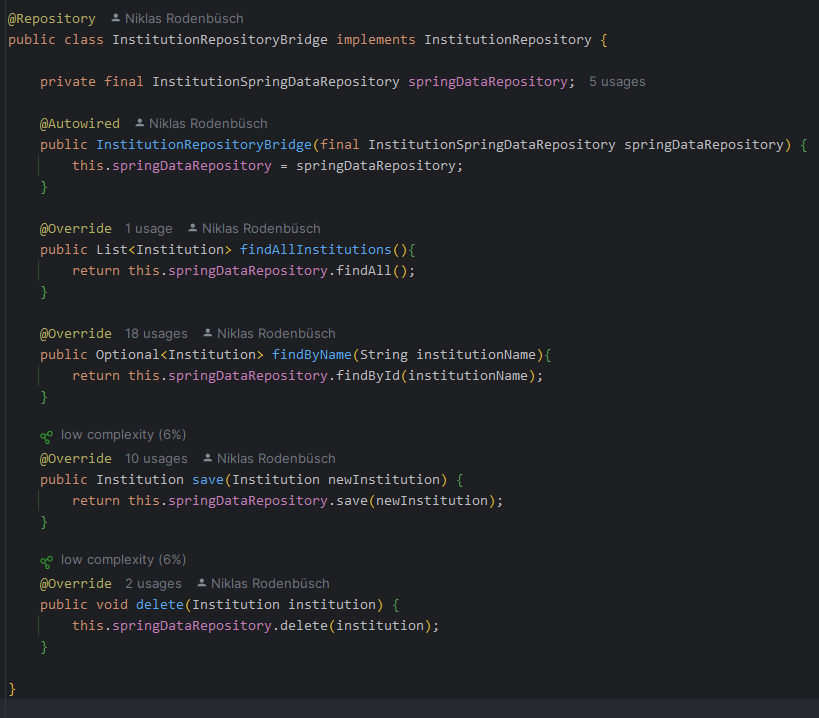
\includegraphics[width=16.5cm]{images/indirection.png}}
    \caption[Indirection Principle]{Indirection principle anhand der Klasse InstitutionRepositoryBridge}
    \label{fig:indirection}
\end{figure}